\documentclass[12pt,a4paper,titlepage]{scrreprt}

% Language is defined in package module

%\usepackage{fontspec}
\usepackage{pdfpages} % For inclusion of PDFs

\usepackage{tabulary}
\usepackage{emoji}

%pro formátování čísel
\usepackage{numprint}
\npthousandsep{\,}\npthousandthpartsep{}\npdecimalsign{.}

\usepackage{xcolor}
\usepackage{soul}
\definecolor{lightgray}{gray}{0.9}
\sethlcolor{lightgray}

%Uprava (odstraneni modifikaci generovaneneho texttu tridou scratcl)
%\setkomafont{disposition}{\mdseries\rmfamily}

\title{\vspace{6cm}Marvus in C++}
\subtitle{Documentation}
\author{Riyufuchi}
\date{\today}

\usepackage[a-1b]{pdfx} % PDF/A-1b compliance
% Ensure metadata is copied correctly
%\immediate\write18{cp pdfa.xmpdata \jobname.xmpdata}

\usepackage{hyperref}

\usepackage{datatool}

\hypersetup{
  %pdfauthor={},
  %pdftitle={Navrh zařízení pro testování nabíjecích kabelů},
  %pdfkeywords={arduino, internet of things, microcontroller, electric energy},
  %pdfsubject={Bakalářská práce},
  %pdfproducer={LaTeX},%
	%pdfcreator={LuaLaTeX}
  colorlinks=true,        % false: boxed links; true: colored links
  linkcolor=black,        % color of internal links
  citecolor=black,        % color of links to bibliography
  filecolor=black,        % color of file links
  urlcolor=black          % color of external links
}

%font
%\usepackage[T1]{fontenc}   % better character encoding
%\usepackage{luainputenc} 
%\usepackage[utf8]{inputenc}
\usepackage{lmodern}       % Latin Modern font
%\setmainfont{Times_New_Roman}
%\usepackage{lmodern}       % Latin Modern font



%Rozestup řádku (1.5)
\linespread{1.35}

%\usepackage{setspace}
%\onehalfspacing

\usepackage{tcolorbox}
\tcbset{
    highlight style/.style={
        colframe=white,
        colback=lightgray,
        boxrule=0pt,
        arc=0pt,
        boxsep=0pt,
        left=0pt,
        right=0pt,
        top=0pt,
        bottom=0pt,
        box align=base
    }
}

%Nastaveni okraje
%\usepackage[a4paper, left=3.50cm, right=1.50cm, top=2.50cm, bottom=2.50cm]{geometry}
\usepackage[a4paper, margin=1in]{geometry}

\RedeclareSectionCommand[
  beforeskip=.1cm,
  afterskip= .1cm %1.0ex plus .2ex
]{chapter}

%\setkomafont{chapter}{\fontsize{18}{18*1.2}\selectfont}
\setkomafont{chapter}{\fontsize{16}{19.2}\selectfont}   
\setkomafont{section}{\fontsize{14}{16.8}\selectfont}
\setkomafont{subsection}{\fontsize{13}{15.6}\selectfont}
\setkomafont{subsubsection}{\fontsize{13}{15.6}\selectfont}

% WIP modules
\usepackage[acronym]{glossaries}
\newglossaryentry{gtk}{name={GTK 4}, description={A cross-platform GUI toolkit}}
\newglossaryentry{wxwidgets}{name={wxWidgets}, description={A cross-platform GUI toolkit for C++}}
\newacronym{gui}{GUI}{Graphical User Interface}
\makeglossaries

% Customize the glossary style to remove page numbers
\newglossarystyle{mystyle}{%
  \renewenvironment{theglossary}%
    {\begin{description}}{\end{description}}%
  \renewcommand*{\glossentry}[2]{%
    \item[\glsentryitem{##1}\glstarget{##1}{\glossentryname{##1}}] %
    \glossentrydesc{##1}\glspostdescription\space}%
}

%\renewcommand{\glossaryname}{}
%\renewcommand{\glossarysection}[2][]{}

\glsaddall
% My modules
\input{tex_modules/czech.tex}
\input{tex_modules/paragraph.tex}
\input{tex_modules/cppListing.tex}
\input{tex_modules/table.tex}
\input{tex_modules/justify.tex}
\input{tex_modules/command-fontSize.tex}
\input{tex_modules/command-figure.tex}

\usepackage{xspace}
% My commands
\newcommand{\wxw}{wxWidgets\xspace}

\newcommand{\TypeTextDB}{\textcolor{blue}{TEXT}}
\newcommand{\TypeRealDB}{\textcolor{purple}{REAL}}
\newcommand{\TypeIntegerDB}{\textcolor{orange}{INTEGER}}
\newcommand{\TypeDateDB}{\textcolor{magenta}{DATE}}


\begin{document}
	
	%\maketitle
	
	\begin{titlepage}
		\begin{center}
			{\Large C++ \& Qt 6} \\
			{\Large ERP Systém}
			\vfill
			{\Huge \textbf{Nocovka}}
			\vfill
		\end{center}
		{\large\textbf{ \today}} \hfill {\large \textbf{Riyufuchi}}
	\end{titlepage}
	
	\pagenumbering{gobble}
	\tableofcontents
	\newpage
	\pagenumbering{arabic}
	
	\clearpage
	\addcontentsline{toc}{section}{Glossary}
	\printglossary[type=main, title=Glossary]
	
	\clearpage
	\addcontentsline{toc}{section}{Acronyms}
	\printglossary[type=\acronymtype, style=mystyle]
	
	%!TeX root =  ../../nocovka.tex

\chapter{Úvod}

%!TeX root =  ../../nocovka.tex

\section{Použité technologie}

\subsection{Qt 6}
Qt 6 je moderní cross-platformní framework pro tvorbu grafických aplikací. 

\subsection{SQLite}
Jednoduchý souborový databázový systém, vhodný pro prototypování a lokální uložení dat.

\subsection{ConsoleLib}
\texttt{ConsoleLib}moje knihovna pro zjednodušení tvorby CLI aplikací. Obsahuje také utility moduly, pro dodržení praktiky DRY napříč mými projekty.

%\subsection{MiniZ}
%MiniZ is simple C library for working with zip files which are used to import data from my Java application to this one. 

%\subsection{Boost}
%The Boost C++ Libraries are open source, peer-reviewed, portable and free. Created by experts to be reliable, skillfully-designed, and well-tested.
%!TeX root =  ../../nocovka.tex

\section{Commiting a git commit}

\begin{table} [H]
	\centering
	\catcode`\-=12
	\begin{tabular}[c]{|| c | c ||}
	\hline
		\multicolumn{2}{||c||}{ \textbf{Commit type cheat table}} \\
	\hline
 		 \textbf{Type} & \textbf{Repository change} \\
	\hline
		\textcolor{purple}{Feat:} & A new feature is added \\
	\hline
		\textcolor{blue}{Fixed:} & A bug is fixed \\
	\hline
		\textcolor{orange}{Docs:} & A documentation is updated \\
	\hline
		\textcolor{black}{Refactor:} & A code change that is not affecting functionality \\
	\hline
		\textcolor{brown}{Test:} & A code change in unit tests \\
	\hline
		\textcolor{gray}{Chore:} & A repository maintenance action \\
	\hline
		\textcolor{magenta}{Version x.y} & When new version is released for clearer commit history \\
	\hline
	\end{tabular}
	\caption{Types of commit headers}
	\label{table:cmtHeaders}
\end{table}
\newpage
%!TeX root =  ../../nocovka.tex

\section{Compilace}

\subsection{Dokumentatace}
\begin{lstlisting}[language=bash, caption={Documentation compilation},  label={lst:docs-compile}]
# Make sure you have LaTeX installed

# On Debian/Ubuntu
sudo apt install texlive-full

# On macOS
brew install --cask mactex

# On Windows
# Get the installer from https://www.tug.org/texlive/windows.html

# Get the repository - how to is in section Git and Make
# Build the PDF documentation
# (CMake runs LaTeX twice so Table of Contents and references are correct)
cd latex-doc/
cmake ..
cmake --build . --target docs
\end{lstlisting}



	%!TeX root =  ../../nocovka.tex

\chapter{Databáze}

%!TeX root =  ../../nocovka.tex

\section{ERD Diagram}

\begin{figure}[H]
	\centering
	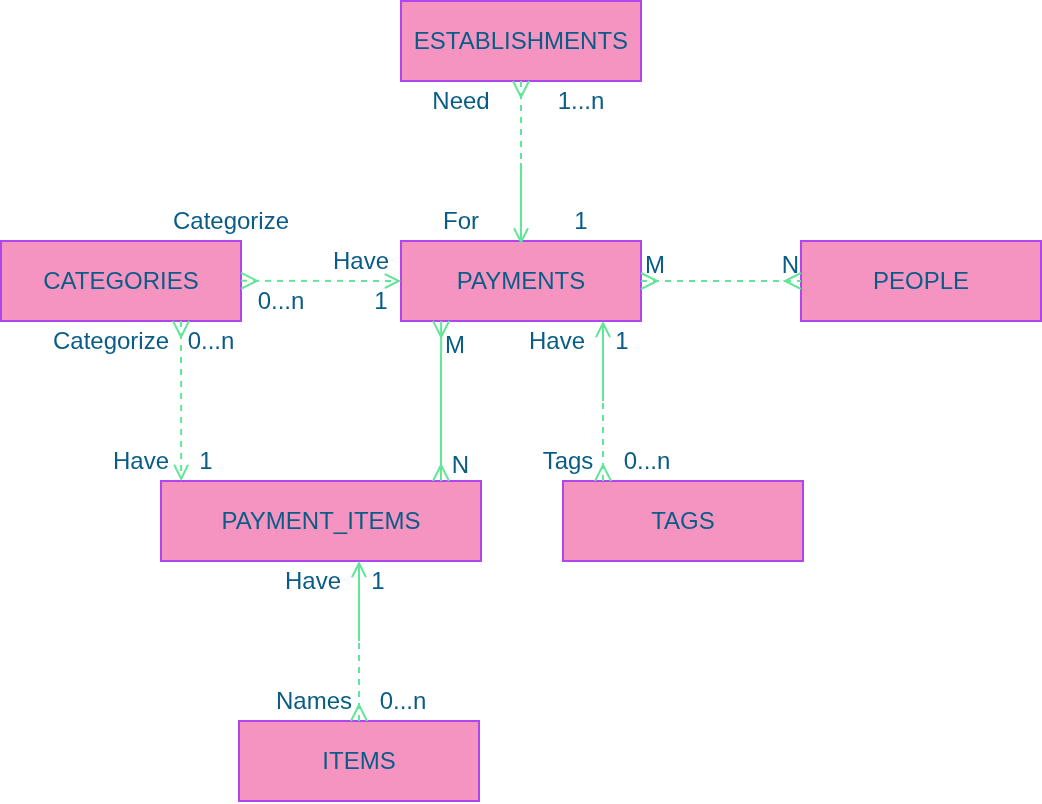
\includegraphics[width=\textwidth]{images/erd.png}
    	\caption{Database ERD}
   	\label{fig:dbERD}
\end{figure}

Each \textbf{PAYMENT} have one  \textbf{CATEGORY} for simplification and this will give us rough statistics per  \textbf{CATEGORY} as
purpose of this database/application is to track income and spending's and not fully accurate accountant statistics.


%!TeX root =  ../../nocovka.tex

\section{Tabulky}

\subsection{PAYMENTS}

\newcolumntype{M}[1]{>{\centering\arraybackslash}m{#1}} % centered vertically

\begin{table}[H]
\centering
\begin{tabulary}{\textwidth}{|| c | c | M{0.55\textwidth} ||}
\hline
    \multicolumn{3}{||c||}{\textbf{Payment table fields}} \\
\hline
    \textbf{Data type} & \textbf{Name} & \textbf{Stores} \\
\hline
    \TypeIntegerDB & payment\_id & Primary key (row identifier). \\
\hline
    \TypeIntegerDB & establishment\_id\_key & Foreign key referencing \texttt{ESTABLISHMENTS} \\
\hline
	\TypeIntegerDB & category\_id\_key       & Foreign key referencing \texttt{CATEGORIES}. \\
\hline
   \makecell[c]{ \TypeTextDB} & payment\_value & Monetary value. Stored as text to avoid loss of decimal precision. \\
\hline
    \makecell[c]{\TypeDateDB} & payment\_date & Date of the payment, stored as string in~ISO-8601 format.* \\
\hline
    \TypeTextDB & payment\_note & Optional free-text note. \\
\hline
\end{tabulary}
\caption{PAYMENTS fields}
\label{table:PAYMENTS}
\end{table}

\noindent\textit{*SQLite does not provide a dedicated \texttt{DATE} type.  
Dates are stored as normalized text in ISO-8601 format (\texttt{YYYY-MM-DD}).}








	
	\chapter*{Závěr}
	
	\newpage
	\addcontentsline{toc}{chapter}{Přílohy}
	\addcontentsline{toc}{section}{Eisenhower matrix}
	\input{chapters/additions/chapter_additions.tex}
	\begin{minipage}{\textwidth}
		
		\addcontentsline{toc}{section}{Listings}
		\lstlistoflistings
		\addcontentsline{toc}{section}{Figures}
		\listoffigures
	 	\addcontentsline{toc}{section}{List of tables}
	 	\listoftables
 	\end{minipage}

\end{document}